\subsection{Application Tuning Parameters} \label{sec:atp}

Applications running on a cluster are aimed to solve numerical problems. Usually, the solutions can be computed with different methods, such as numerical integration (Simpson, Gaussian Quadrature, Newton-Cotes, ...), function minimization (Gradient Descent, Conjugate Gradient Descent, Newton, ...), or finding the eigenvalues and eigenvectors of real matrices (power method, inverse power method, Arnoldi, ...). These methods may have different implementations, like the Fast Fourier Transform (algorithms from Cooley-Tukey, Bruun, Rader, Bluestein) implemented in the FFTW, FFTS, FFTPACK or MKL.

For a given problem, several methods can provide similar numerical solutions through different implementations. In HPC, the developer chooses the most efficient one in terms of numerical accuracy and time to solution. However, the selection also depends on the computer's architecture. For example, some methods can be more efficient on a vector processor than on a superscalar processor. It is up to the application's developer to choose the appropriate method and its implementation that fulfill the computer's specificity.

In the context of energy saving, the energy consumption must also be minimized. This makes it hard for the developer to choose which method and implementation must be executed. READEX offers the developer to expose the various methods and their implementation via Application Tuning Parameters (ATP) to the tuning process. ATPs are communicated to READEX through an API that is used to annotate the source code at locations where the tuning parameters play a role.

\begin{figure}
\centering
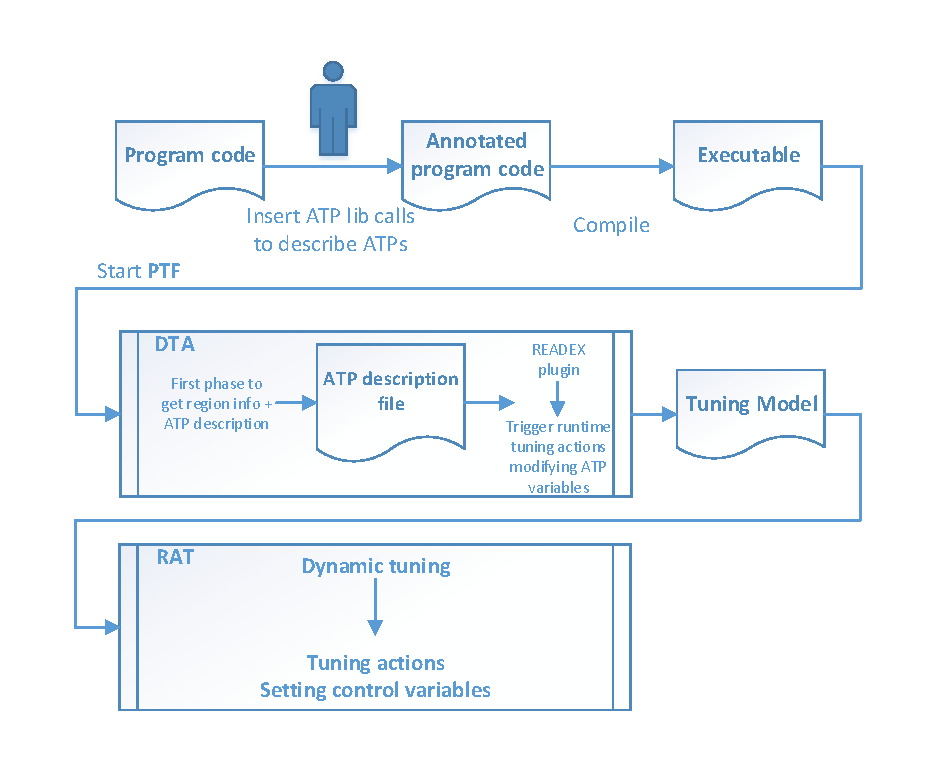
\includegraphics[width=0.8\columnwidth]{figures/overall_design.pdf} 
\caption{Workflow showing the handling of the ATPs in READEX. }
\label{fig_ATP_workflow}
\end{figure} 

Figure~\ref{fig_ATP_workflow} illustrates the steps performed to tune the ATPs. First, ATPs are declared in the code through annotations. The application is then linked against the ATP library, which implements the API. During DTA, the ATP description file is generated by the ATP library. This file includes the tuning parameters with their specifications, and is used to define the search space. The \texttt{readex\_intraphase} tuning plugin extends the search space with the ATPs, and finds the best settings. Finally, the best configurations are stored in the ATM and passed to RAT.

To annotate the code, the application developer exposes control variables and mark them as ATPs with the API functions as illustrated in Listing~\ref{lbl:atp_example}. The function \texttt{ATP\_PARAM\_DECLARE} declares the parameter's name, type, default value and domain. The function \texttt{ATP\_PARAM\_ADD\_VALUES} allows to add possible values the parameter can take, in a range specified by minimal, maximal and increment values or by enumerating explicitly the possible values. The function \texttt{ATP\_PARAM\_GET} fetches the value given in the ATM from the RRL and assigns it to the control variable. 

Several ATPs can be defined in the same code. They may be independent or not. In the latter case, there is a notion of constraints between the parameters. To indicate to READEX that parameters have constraints between them, these parameters are put in the same \textit{domain name}.

Once the source code is annotated and the compiled code is executed, the ATP library generates a description file in which the ATPs are written. This file contains the details about the declared application parameters.

During DTA, PTF launches the ATP server that reads the ATP description file. The ATP server's task is to respond to PTF requests, such as providing the list of ATPs or a list of valid values of the ATPs. The \texttt{readex\_intraphase} tuning plugin uses the list of valid values to generate a search space of the tuning parameters (not only the ATPs) and explore it. The resulting tuning model also consists of the best combination of the ATPs.
\newpage

\definecolor{mygray}{rgb}{0.46,0.46,0.46}
\lstset{language=[90]Fortran,
	%	basicstyle=\ttfamily,
	frame=lines,
	xleftmargin=\parindent,
	aboveskip=2mm,
	belowskip=2mm,
	showstringspaces=false,
	columns=flexible,
	breaklines=true,
	breakatwhitespace=true,
	keywordstyle=\color{blue},
	commentstyle=\color{mygray},
	numbers=left,
	numberstyle=\tiny\color{mygray},
	numbersep=1em,
	escapeinside={(@*}{*@)},
}

%\begin{multicols}{2}[\captionof{lstlisting}{ATP constraint and exploration declaration with the ATP library.}] \label{lbl:atp_example}
%\begin{lstlisting}[language=C,xleftmargin=3em,frame=none,title=\phantom{xxx}]
%void foo(){
%  int atp_cv;
%  ...
%  ATP_PARAM_DECLARE("solver", RANGE, 1, "DOM1");
%  int32_t solver_values[3] = {1,5,1};
%  ATP_ADD_VALUES("solver", solver_values, 3, "DOM1");
%  ATP_PARAM_GET("solver", &atp_cv, "DOM1");
%	
%  switch (atp_cv){
%  case 1:
%    // choose solver 1
%    break;
%  case 2:
%    // choose solver 2
%    break;
%    ...
%  }
%  int32_t hint_array = {GENETIC, RANDOM};
%  ATP_EXPLORATION_DECLARE(hint_array, "DOM1");
%}
%	
%void bar(){
%  int atp_ms;
%  ...
%  ATP_PARAM_DECLARE("mesh", RANGE, 40, "DOM1");
%  int32_t mesh_values[3] = {0,80,10};
%  ATP_ADD_VALUES("mesh", mesh_values, 3, "DOM1");
%  ATP_PARAM_GET("mesh", &atp_ms, "DOM1");
%  ATP_CONSTRAINT_DECLARE("const1", "(solver = 1 && 0 <= mesh <= 40) || (solver = 2 && 40 <= mesh <= 80) || (solver > 2 && mesh = 120)", "DOM1");
%  if((atp_ms > 1) && (atp_ms <= 40)){
%    // choose mesh size 1
%  }
%  if((atp_ms > 40) && (atp_ms <= 80)){
%    // choose mesh size 2
%  }
%  if(atp_ms == 120){
%    // choose mesh size 3
%  }
%}
%\end{lstlisting}
%\end{multicols}

\begin{lstlisting}[language=C,xleftmargin=3em,frame=none,title=\phantom{xxx},caption=ATP constraint and exploration declaration with the ATP library.,label=lbl:atp_example]
void foo(){
  int atp_cv;
  ...
  ATP_PARAM_DECLARE("solver", RANGE, 1, "DOM1");
  int32_t solver_values[3] = {1,5,1};
  ATP_ADD_VALUES("solver", solver_values, 3, "DOM1");
  ATP_PARAM_GET("solver", &atp_cv, "DOM1");
	
  switch (atp_cv){
  case 1:
    // choose solver 1
    break;
  case 2:
    // choose solver 2
    break;
    ...
  }
  int32_t hint_array = {GENETIC, RANDOM};
  ATP_EXPLORATION_DECLARE(hint_array, "DOM1");
}
	
void bar(){
  int atp_ms;
  ...
  ATP_PARAM_DECLARE("mesh", RANGE, 40, "DOM1");
  int32_t mesh_values[3] = {0,80,10};
  ATP_ADD_VALUES("mesh", mesh_values, 3, "DOM1");
  ATP_PARAM_GET("mesh", &atp_ms, "DOM1");
  ATP_CONSTRAINT_DECLARE("const1", "(solver = 1 && 0 <= mesh <= 40) || (solver = 2 && 40 <= mesh <= 80) || (solver > 2 && mesh = 120)", "DOM1");
  if((atp_ms > 1) && (atp_ms <= 40)){
    // choose mesh size 1
  }
  if((atp_ms > 40) && (atp_ms <= 80)){
    // choose mesh size 2
  }
  if(atp_ms == 120){
    // choose mesh size 3
  }
}
\end{lstlisting}

The \texttt{readex\_intraphase} plugin provides two new search strategies, \linebreak \texttt{exhaustive\_atp} and \texttt{individual\_atp} to compute the optimal ATP configuration. These two search strategies can also be configured via the READEX configuration file.

The \texttt{exhaustive\_atp} search space is built from the cross-product of all valid combinations of ATPs. The plugin contacts to the ATP server to receive the valid combinations of the points for each of the given ATP domains. The configuration set is then built from the cross-product of the computed valid points. 

On the other hand, the \texttt{individual\_atp} strategy tunes the domains individually. It first evaluates all valid points for the first domain. The best point from this domain remains fixed and the next domain is investigated until all the domains are explored.  

The tuning of ATPs is done before the tuning of the frequencies and the threads since it determines the algorithm to be used during execution. This algorithm is then tuned in subsequent tuning steps of the \texttt{readex\_intraphase} tuning plugin with respect to the system and runtime parameters. 

The best configuration of the ATPs is finally passed to RAT through the ATM as any other tuning parameter. At runtime, the optimal value is read through the ATP library in combination with the RRL and is assigned to the control variable.
